\section{Chronologie}%\addcontentsline{toc}{section}{Chronologie}
\fancyhead[RO]{Chronologie}
% \fancyhead[LO]{}

    Die \ceva{c-base} ist eine abgestürzte Raumstation (\cevain{c-tation}) unter Berlin, die sich seit 1995 rekonstruiert~\cite{cbasebook}. Dieser Prozess ist auch bekannt als \cevain{cbrp},  eine Abkürzung für \cevain{c-base reconstruction project}. 
    
    Zur besseren Einordnung unterscheiden wir in enger Anlehnung an \cite{cbasepressemap} und \cite{cbasebook} folgende Epochen der Stationsgeschichte:
    % \twofonts{
    \begin{enumerate}
        \item \textbf{Unzeit:} vor dem Absturz 4,5 Milliarden \textsc{bp}  (\emph{before present}), identisch mit der \textbf{Fernen Zukunft:} ursprüngliche bzw. zukünftige Konstruktion der \ceva{c-base}.
        
        \item \textbf{Urzeit} bzw. \cevain{dark age}. Beginnt mit dem  Absturz 4,5 Milliarden \textsc{bp}  und endet mit dem eigenständigen Einschalten des Bordcomputers \cevain{c-beam} \cite{cbasepressemap} 100.000 \textsc{bp} .
        
        \item \textbf{Keimzeit:} beginnt mit dem Wiedereinschalten von \ceva{c-beam} 100.000 \textsc{bp}  Erste Periode des \cevain{reconstruction age}; erste Schritte der Selbstrekonstruktion. Ende mit der Sichtbarwerdung der Antenne 1965.
        
        \item \textbf{Vorzeit:} beginnt mit der Sichtbarwerdung der Antenne 1965. Erste Inspiration von Karboneinheiten durch \ceva{c-beam}. Vorschriftliche Periode. Mythische Periode; vermutlich erste Zusammenkünfte der \cevain{gründer} (\cref{tab:gruender}). Endet mit der Auffindung des \cevain{urartefact} 1995.
        
        \item \textbf{Archaische Zeit:} \cevain{cbrp1}. Beginnt mit der Auffindung des \ceva{urartefact} im Februar 1995.  Nachbau und Rekonstruktion einer Schleusensektion auf 270$m^2$ in der Oranienburger Str. 2. \cite{cbasepressemap}~\cite{cbasebook}. Heldenzeit; Erscheinen von \cite{cbaselogbuchpre} und \cite{cbaselogbuchnow}. Endet mit dem Umzug in die Rungestr. 20 im Mai 2000.
        
        \item \textbf{Frühzeit:} - \cevain{cbrp2}. Beginnt mit dem Umzug in die Rungestr. 20 im Juni 2000.  Nachbau und Rekonstruktion einer Multimodulstation \ceva{RS20} auf 524$m^2$ in der Rungestr. 20~\cite{cbasepressemap}~\cite{cbasebook}. Ende mit dem Umzug an den Franz-Mehring-Platz Nr. 1 im August 2002.
        
        \item \textbf{Zwischenzeit:}  \cevain{c-visiondecc} / \cevain{cwischendecc}.  Beginnt mit dem Umzug an den Franz-Mehring-Platz Nr. 1 im September 2002. 
        Auslagerung wegen Wartungsarbeiten in der \ceva{RS20}.~\cite{cbasepressemap}~\cite{cbasebook}.  Endet mit dem Rücksturz in die Rungestr. im Julie 2003.
        
        \item \textbf{Mittelalter:}  \cevain{cbrp3a}. Beginnt mit dem Rücksturz in die Rungestr. 20 im August 2003. 
         Erweiterung der Fläche auf ca. 720$m^2$ auf 2 Etagen. Fortgesetzte Konstuktion \cite{cbasepressemap}~\cite{cbasebook}. Erscheinen von \cite{cbasestarbasemanual} und \cite{ctour}. Diese Epoche endet 2015 mit dem Erscheinen des \ceva{c-booc}).
        
         \item \textbf{Neuzeit:} \cevain{cbrp3b}. Beginnt 2015 mit dem Erscheinen des \ceva{c-booc}, das den Kanon abschließt. Verfeinerung und Dekadenz. Verinnerlichung, Selbstbewusstwerdung. Mission und Ausgründungen. Die Epoche endet mit dieser Veröffentlichung, mit der die Gegenwart beginnt.
    \end{enumerate}
    % }


\begin{figure}
    \centering
        % \documentclass{standalone}
\usepackage{tikz}
\usepackage{fontspec}

\newcommand{\ceva}[1]{ {\fontspec{[ceva-c2.ttf]}#1}}
\newcommand{\cevain}[1]{ {\fontspec{[ceva-c2.ttf]}#1} | \emph{#1}}

\begin{document}
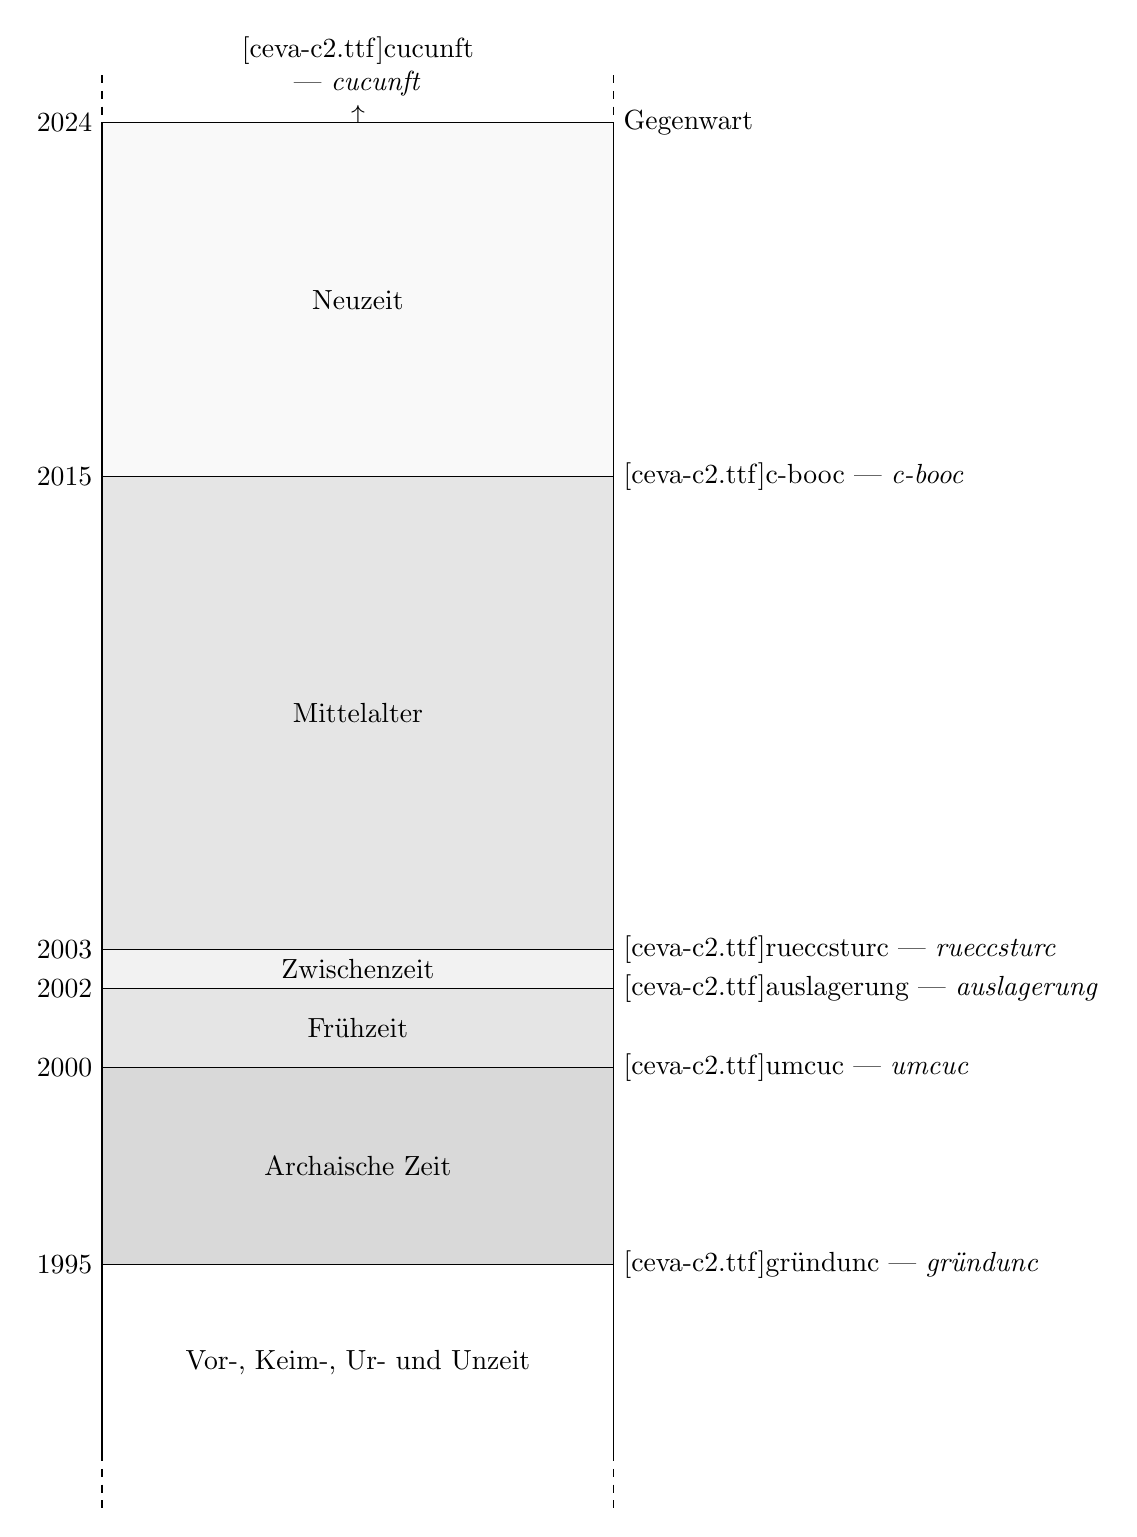
\begin{tikzpicture}[yscale=0.5,xscale=1.3]
    % \draw (0) rectangle (0,,1);
    \foreach \i in {124.4,124.8,125.2} 
        {
        \draw (0,\i) -- (0,\i-0.2);
        \draw (5,\i) -- (5,\i-0.2);
        }

    \node at (2.5,125) {\parbox{20ex}{\centering\cevain{cucunft}\\ $\uparrow$ }};
    
    \node [right] at (5,124) {Gegenwart};
    
    \draw[fill=gray!5] (0,124) node [left] {2024} rectangle node {Neuzeit} (5,115) node [right] {\cevain{c-booc}};
    % \draw (0,115) -- (0,124); draw (5,114) -- (5,124); \draw (0,115
    
    \draw[fill=gray!20] (0,115) node [left] {2015} rectangle node {Mittelalter} (5,103) node [right] {\cevain{rueccsturc}};
    
    \draw[fill=gray!10] (0,103)  node [left] {2003} rectangle node {Zwischenzeit} (5,102) node [right] {\cevain{auslagerung}};
    
    \draw[fill=gray!20] (0,102)  node [left] {2002} rectangle node {Frühzeit} (5,100) node [right] {\cevain{umcuc}};
    
    \draw[fill=gray!30] (0,100)  node [left] {2000} rectangle node {Archaische Zeit} (5,95) node [right] {\cevain{gründunc}};
    % \node at (0,95) [left] {1995};
    
    \draw[draw=none] (0,95)  node [left] {1995} rectangle node {Vor-, Keim-, Ur- und Unzeit} (5,90) ;
    \draw (0,95) -- (0,90); \draw (5,95) -- (5,90);
    
    \foreach \i in {89.8,89.4,89} 
        {
        \draw (0,\i) -- (0,\i-0.2);
        \draw (5,\i) -- (5,\i-0.2);
        }
    
    
    % \draw[<->] (0,95) rectangle (0,65);
\end{tikzpicture}

\end{document}

        \resizebox{\textwidth}{!}{
        \documentclass{standalone}
\usepackage{tikz}
\usepackage{fontspec}

\definecolor{eins}{HTML}{e7e7e8}   %% Ring 1 "core"     - weiß - Mittelpunkt, Ring um Mittelpunkt
\definecolor{zwei}{HTML}{ed1c24}   %% Ring 2 "com"      - rot -  "Fenster" innen
\definecolor{drei}{HTML}{fbad18}   %% Ring 3  "culture" - orange - fünf Module, quasi invertiert
\definecolor{vier}{HTML}{74c043}   %% Ring 4  "creactiv" - grün -  vier Module
\definecolor{fuenf}{HTML}{0089d0}  %% Ring 5 "cience"  - cyan (blau) - drei Module mit "Strich"
\definecolor{sechs}{HTML}{11357e}  %% Ring 6 "carbon" -  indigo - viele "Fenster" außen
\definecolor{sieben}{HTML}{000000} %% Ring 7 "clamp" -  schwarz, c-förmig
\definecolor{cbase}{HTML}{222222}  %% Körper der Raumstation    

\newcommand{\ceva}[1]{ {\fontspec{[ceva-c2.ttf]}#1}}
\newcommand{\cevain}[1]{{ \fontspec{[ceva-c2.ttf]}#1} | \emph{#1}}

\begin{document}
\begin{tikzpicture}[yscale=2.4,xscale=-0.5,rotate=90,
    every node/.style={
        fill=white,font=\sffamily 
        }
    ]
    % \draw (0) rectangle (0,,1);
    \foreach \i in {124.4,124.8,125.2} 
        {
        \draw (0,\i) -- (0,\i-0.2);
        \draw (5,\i) -- (5,\i-0.2);
        }

    \node [right] at (2.5,124) {$\rightarrow t$  };
    
    \node [below left,rotate=90] at (5,124) {\footnotesize Gegenwart};
    
    \draw[fill=eins!5] (0,124) node [left, rotate=90]{2024} rectangle node {Neuzeit} (5,115) node [below left,rotate=90] {\footnotesize\cevain{c-booc}};
    % \draw (0,115) -- (0,124); draw (5,114) -- (5,124); \draw (0,115
    
    \draw[fill=zwei!20] (0,115) node [left, rotate=90]{2015} rectangle node {Mittelalter} (5,103) node [below left,rotate=90] {\footnotesize\cevain{rueccsturc}};
    
    \draw[fill=drei!10] (0,103)  node [left, rotate=90]{2003} rectangle   (5,102) node [below left,rotate=90] {\footnotesize\cevain{auslagerung}};
    
    \draw[fill=vier!20] (0,102)  node [left, rotate=90]{2002} rectangle (5,100) node [below left,rotate=90] {\footnotesize\cevain{umcuc}};

    
    \draw[fill=fuenf!30] (0,100)  node [left, rotate=90]{2000} rectangle node {Archaik} (5,95) node [below left,rotate=90]{\footnotesize\cevain{gründunc}};
    % \node at (0,95) [left] {1995};
    
    \draw[fill=sechs!5,draw=none] (0,95)  node [left, rotate=90]{1995} rectangle node[text width=8ex,align=center] {Vor-, Keim-, Ur- und Unzeit} (5,90) ;
    \draw (0,95) -- (0,90); \draw (5,95) -- (5,90);
    
    \foreach \i in {89.8,89.4,89} 
        {
        \draw (0,\i) -- (0,\i-0.2);
        \draw (5,\i) -- (5,\i-0.2);
        }

    \node at (2.1,101) {Frühzeit};
    \node [text width=9ex, align=center] at (1.5,102.5) {Zwischen-\\zeit};
    
    % \draw[<->] (0,95) rectangle (0,65);
\end{tikzpicture}

\end{document}

        }
        \vspace{2ex}
    \caption{Periodisierung der Rekonstruktionsgeschichte}
    \label{fig:perioden}
\end{figure}

Eine Überblick über die Dauer der einzelnen Perioden gibt \cref{fig:perioden}. Zur Urzeit siehe~\cite{cbaselogbuchpre}. Aus der Vorzeit liegen überwiegend inspirierte literarische Werke vor (z.B.~\cite{rfc968cerf}, \cite{rfc527cerf}). Zur Archaischen Zeit der Station siehe~\cite{cbaselogbuchnow} mit Einträgen 1995-1999.


Der rezente Zustand und Befund ihrer Vorzeit sowie Zukunft ist vor allem in \cite{cbasebook} beschrieben, aber auch in weiteren Veröffentlichungen wie etwa \cite{cbasewebsite}. Der aktuelle Rekonstruktionsstand lässt sich in der Rungestraße besichtigen; die früheren Ausgrabungen sind leider wieder verschüttet worden. Im Folgenden werten wir die vorhandenen historischen (schriftlichen) Quellen  aus. Diese stammen überwiegend aus der Frühen Neuzeit mit deutlichen Wurzeln in früheren (bzw. späteren) Zeitaltern.

\begin{table}[ht!]
    \centering
    \begin{tabular}{r|l}
    % \cevain{
    \toprule
        \ceva{cynk}& \emph{cynk} \\
        \ceva{mars}& \emph{mars} \\
        \ceva{nomax}& \emph{nomax } \\
        \ceva{hein-c}& \emph{hein-c } \\
        \ceva{biafra}& \emph{biafra} \\
        \ceva{c\_ana}& \emph{c\_ana} \\
        \ceva{lester}& \emph{lester} \\
        \ceva{antenne}& \emph{antenne} \\
        \ceva{tmf powersau}& \emph{tmf powersau} \\
        \ceva{mash}& \emph{mash} \\
        \ceva{westcar}& \emph{westcar} \\
        \ceva{alex}& \emph{alex} \\
        \ceva{olli}& \emph{olli} \\
        \ceva{wallner}& \emph{wallner} \\
        \ceva{gerhard}& \emph{gerhard} \\
         % \cevain{cynk}\\ \cevain{mars}\\  \cevain{nomax}\\  \cevain{hein-c}\\  \cevain{biafra}\\  \cevain{c\_ana}\\  \cevain{lester}\\  \cevain{antenne}\\  \cevain{tmf powersau}\\  \cevain{mash}\\  \cevain{westcar}\\  \cevain{alex}\\  \cevain{olli}\\  \cevain{wallner}\\  \cevain{gerhard}\\
    \bottomrule
    % }
    \end{tabular}
    
    \caption{Die 15 \cevain{gründer}}
    \label{tab:gruender}
\end{table}

% Da wir hier eine Quellenanalyse 

